\section{28. November 2018}
%! Hier gibts schon ein bisschen was hier: https://docs.google.com/document/d/1VvuRhqSy6umcpChijdMtuYw5qB0H7iJZGPXQbSMj6zA/edit
\question{Skizzieren Sie die wesentlichen Elemente der Born-Oppenheimer Näherung.}
\label{q:61}

Da die Atomkerne eine wesentlich größere Masse als die Elektronen haben und sich dadurch viel langsamer bewegen, ist es mit der Born-Oppenheimer
Näherung möglich die Positionen der Kerne zu fixieren. Somit lässt sich die molekulare Schrödingergleichung in eine für die Kerne und eine
für die Elektronen aufteilen.

\begin{itemize}
    \item Für die Elektronen stehen die Kerne still, wodurch ihre Lage als Parameter in das anziehende und abstoßende Potential eingeht.
        Somit hängen die elektronischen Eigenzustände und Energien nur von der Lage der Kerne ab und nicht von der Geschwindigkeit.\\
            Die Schrödingergleichung für die Elektronen lautet somit:
            
        \begin{align}
            \hat{H}_e * \Phi_h(\vec{r},\vec{R}) = E_h(\vec{R}) *  \Phi_h(\vec{r},\vec{R})
        \end{align}

        Dabei ist $\vec{r}$ die Position der Elektronen und $\vec{R}$ die der Kerne. Der Hamiton besteht aus $\hat{H}_e = \hat{T}_e + \hat{V}_{ee} + \hat{V}_{eN}$, 
        also der kinetischen Energie der Elektronen + der Abstoßung zwischen den Elektronen + der Anziehung zwischen Kernen und Elektronen.

        \begin{figure}[H]
            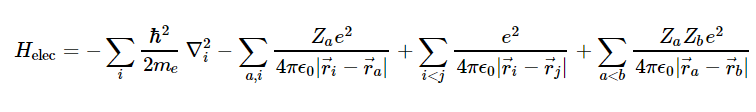
\includegraphics[width=0.8\linewidth]{resources/09-05-2012/born_op.PNG}
            \caption{Elektronischer Hamiton}
        \end{figure}

    \item Die Kernbewegeung ist von den Elektronen nahezu unbeeinflusst, jedoch bewegen sie sich im Potential der elektrischen Zustände. 
        Die Kern-Wellenfunktion $\eta_{hk}(\vec{R})$ hängt nur von der Kernkoordinate $\vec{R}$ ab.\\
        Die Schrödingergleichung lautet: 

        \begin{align}
            (\hat{T}_n + \hat{V}_{NN} + E_h(\vec{R})) * \eta_{hk}(\vec{R}) = E_{hk} * \eta_{hk}(\vec{R})
        \end{align}
\end{itemize}


\question{Diskutieren Sie die sp-, sp2-, sp3-Hybridisierung in mehratomigen Molekülen.}
\label{q:62}

Hybridisierung bedeutet eine Mischung aus s- und p- Orbitalen,
hervorgerufen durch die Verformung der Elektronenhülle auf Grund
der Wechselwirkung zwischen den an der Bindung beteiligten Atomen.
Dabei gibt es die sp-, die sp2- und die sp3-Hybridisierung:

\begin{itemize}
    \item Eine sp-Hybridisierung führt zu zwei entgegengerichteten Bindungen und damit
          zu einem linearen Molekül, wenn keine anderen Bindungen vorhanden sind. Hier hybridisieren das 2s und ein 2p Orbital zu zwei sp-Orbitalen.
         
          \begin{figure}[H]
            \begin{minipage}[b]{0.5\linewidth} 
               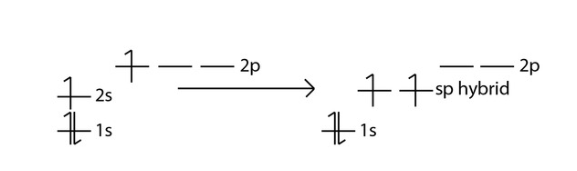
\includegraphics[width=0.8\linewidth]{resources/28-11-2018/sp11.PNG}
               \caption{sp-Hybridisierung, wobei die Energie sinkt}
            \end{minipage}
            \hspace{0.01\linewidth}
            \begin{minipage}[b]{0.5\linewidth} 
               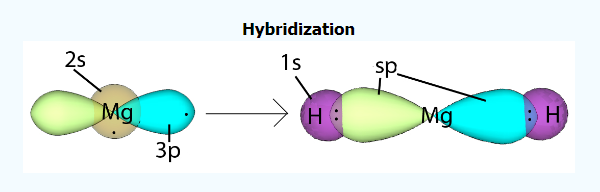
\includegraphics[width=0.8\linewidth]{resources/28-11-2018/sp12.PNG}
               \caption{sp-Hybridisierung am Beispiel von Magnesium }
            \end{minipage}
         \end{figure}

    \item Die sp2-Hybridisierung führt zu drei gerichteten Bindungen, die in einer
          Ebene liegen. Hier bilden sich aus den 2s und zwei 2p-Orbitalen, drei sp-Orbitale.

          \begin{figure}[H]
            \begin{minipage}[b]{0.5\linewidth} 
               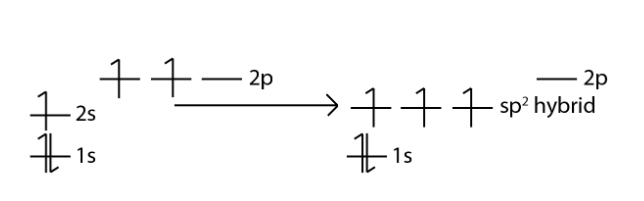
\includegraphics[width=0.8\linewidth]{resources/28-11-2018/sp21.PNG}
               \caption{sp2-Hybridisierung, wobei die Energie sinkt}
            \end{minipage}
            \hspace{0.01\linewidth}
            \begin{minipage}[b]{0.5\linewidth} 
               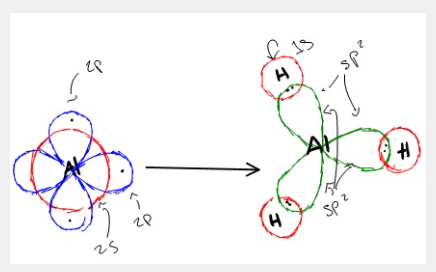
\includegraphics[width=0.8\linewidth]{resources/28-11-2018/sp22.PNG}
               \caption{sp2-Hybridisierung am Beispiel von Aluminiumhydroxid}
            \end{minipage}
         \end{figure}

    \item Für die sp3-Hybridisierung ergeben sich Atomorbitale mit Maxima, die in die vier Ecken eines Tetraeders zeigen.
          Hier bilden sich aus den 2s und drei 2p-Orbitalen, vier sp3-Orbitale.

          \begin{figure}[H]
            \begin{minipage}[b]{0.5\linewidth} 
               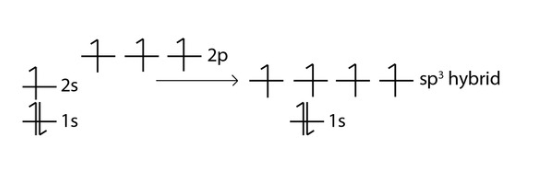
\includegraphics[width=0.8\linewidth]{resources/28-11-2018/sp31.PNG}
               \caption{sp3-Hybridisierung, wobei die Energie sinkt}
            \end{minipage}
            \hspace{0.01\linewidth}
            \begin{minipage}[b]{0.5\linewidth} 
               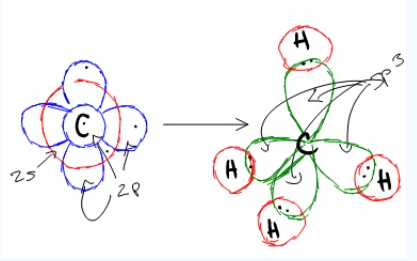
\includegraphics[width=0.8\linewidth]{resources/28-11-2018/sp32.PNG}
               \caption{sp3-Hybridisierung am Beispiel von Methan}
            \end{minipage}
         \end{figure}

\end{itemize}

\question{Diskutieren Sie die Laue'sche Beugungsbedingung anhand der Ewald-Konstruktion im Rahmen der Bragg'schen Interpretation.}
\label{q:63}

\question{Wodurch unterscheiden sich ein fcc-Gitter von einer hcp-Struktur?}
\label{q:64}

siehe \aqref{46}

\question{Diskutieren Sie die Gitterenergie der Ionenkristalle.}
\label{q:65}

\question{Vergleichen Sie die Einstein- und Debye-Modelle der spezifischen Wärme. Welche Annahmen sind in beiden Modellen zu einfach?}
\label{q:66}

\question{Diskutieren Sie das Auftreten einer Energiebandlücke mit Hilfe des Modells der fast freien Elektronen.}
\label{q:67}

siehe \aqref{5}

\question{Wodurch unterscheidet sich die Dispersionsrelation der Phononen eines primitiven kubischen Gitters von jenem eines CsCl-Gitters.}
\label{q:68}

\question{Erklären Sie die chemische Bindung von $O_2$ (O; $Z=8$).}
\label{q:69}

Elektronenkonfiguration O$_2$: $1\sigma_g^2 ~ 1\sigma_u^{*2} ~ 2\sigma_g^2 ~ 2\sigma_u^{*2} ~ 1\pi_u^4 ~ 3\sigma_g^2 ~ 1\pi_u^4 ~ 1\pi_g^2$ \\

Da beide Sauerstoffatome je zwei freie Elektronenpaare haben, kommt es zu einer Doppelbindung.

\begin{figure}[H]
    \begin{minipage}[b]{0.5\linewidth} 
       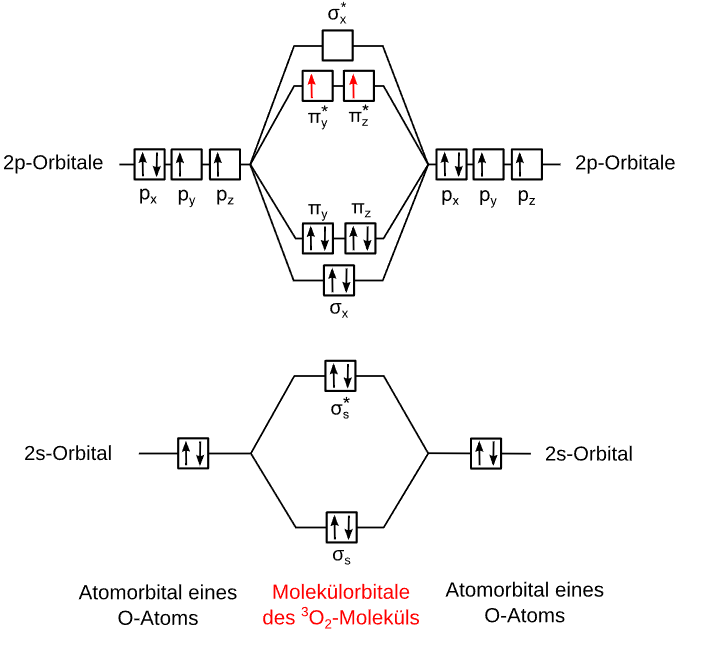
\includegraphics[width=0.8\linewidth]{resources/28-11-2018/O2.PNG}
       \caption{Elektronenkonfiguration von $O_2$}
    \end{minipage}
    \hspace{0.01\linewidth}
    \begin{minipage}[b]{0.5\linewidth} 
       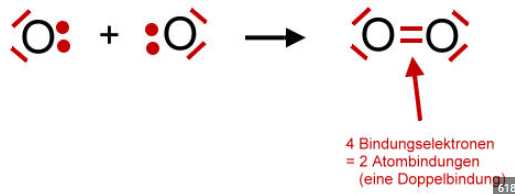
\includegraphics[width=0.8\linewidth]{resources/28-11-2018/o2_bindung.PNG}
       \caption{Chemische Bindung zweier Sauerstoffatome}
    \end{minipage}
 \end{figure}

\newpage